\chapter{Results} \label{sec:results}

\section{The First Trimming Strategy } \label{sec:1st_trimming_stratrgy}

The initial phase of our \gls{assembly} Investigation centered on applying a pipeline \gls{trimming} Strategy, herein referred to as the "First \gls{trimming} Strategy." (\autoref{tab:trimming_results_first}). This approach was designed to set a standard against which we could measure the effectiveness of subsequent \gls{trimming} Methods. Our primary objective was to assess its impact on crucial \gls{assembly} Metrics. The First \gls{trimming} Strategy was implemented with conservative parameters aimed at minimal data loss while ensuring the removal of low-quality sequences. This phase was critical for establishing a control scenario, providing us with a benchmark for evaluating the efficiency and precision of our \gls{assembly} Process.

\begin{table}[h!]
\centering
\caption{The First Trimming Strategy and Its Impact on Assembly Metrics}
\label{tab:trimming_results_first}
\resizebox{\textwidth}{!}{
\begin{tabular}{|c|l|r|r|r|r|r|r|r|r|}
\hline
\textbf{\#} & \textbf{Trimming Parameters} & \textbf{Total length} & \textbf{GC (\%)} & \textbf{Largest Contig} & \textbf{N50} & \textbf{N90} & \textbf{L50} & \textbf{L90} & \textbf{\# N's per 100 kbp} \\ \hline
0 & NoTrimming & 4404338 & 65.49 & 209132 & 74608 & 21687 & 18 & 57 & 9.20 \\
1 & QualityTrim\_Q25 & 4347132 & 65.39 & 206803 & 64262 & 17217 & 20 & 68 & 7.43 \\
2 & AdapterTrim\_Q25 & 4347132 & 65.39 & 206803 & 64262 & 17217 & 20 & 68 & 7.43 \\
3 & LengthFilter\_75 & 4371727 & 65.42 & 209097 & 65136 & 17421 & 19 & 64 & 6.94 \\
4 & ComplexityFilter & 4370526 & 65.41 & 209097 & 65136 & 17421 & 19 & 64 & 6.94 \\
5 & SlidingWindow\_4nt\_q25 & 4338271 & 65.45 & 173819 & 56417 & 16144 & 26 & 81 & 7.86 \\
6 & QualitySlidingHybrid\_Q25\_4nt\_q25 & 4338271 & 65.45 & 173819 & 56417 & 16144 & 26 & 81 & 7.86 \\
7 & QualityAdapterHybrid\_Q25 & 4347132 & 65.39 & 206803 & 64262 & 17217 & 20 & 68 & 7.43 \\
8 & LengthComplexityHybrid\_75 & 4371727 & 65.42 & 209097 & 65136 & 17421 & 19 & 64 & 6.94 \\
9 & SlidingComplexityHybrid\_4nt\_q25 & 4338271 & 65.45 & 173819 & 56417 & 16144 & 26 & 81 & 7.86 \\
10 & AdapterSlidingHybrid\_Q25\_4nt\_q25 & 4338271 & 65.45 & 173819 & 56417 & 16144 & 26 & 81 & 7.86 \\
11 & QualityLengthHybrid\_Q25\_75 & 4348087 & 65.39 & 206803 & 64262 & 17217 & 20 & 69 & 7.42 \\
12 & QualityComplexityHybrid\_Q25 & 4348353 & 65.39 & 206803 & 64262 & 17387 & 20 & 67 & 7.43 \\
13 & AdapterLengthHybrid\_Q25\_75 & 4348087 & 65.39 & 206803 & 64262 & 17217 & 20 & 69 & 7.42 \\
14 & AdapterComplexityHybrid\_Q25 & 4348353 & 65.39 & 206803 & 64262 & 17387 & 20 & 67 & 7.43 \\
15 & LengthSlidingHybrid\_75\_4nt\_Q25 & 4315732 & 65.40 & 173819 & 54049 & 16002 & 27 & 84 & 9.06 \\
\hline
\end{tabular}
}
\end{table}

\textit{The data in the \autoref{tab:trimming_results_first} results from reports generated by the first run of the pipeline (\autoref{sec:generated_data}), its extraction with the \autoref{lst:extracting_metrics} calling the \autoref{lst:extraction-function}, and sorting by using the \autoref{lst:sorting_extracted_metrics}, described in the  \autoref{sec:data_extraction}.}


\subsection{Data Normalization}

Subsequently, the task was set to rethink the visualization of the aforementioned data, aiming for a clearer representation (\autoref{fig:genome_assembly_metrics_heatmap_1}). This work started with the definition of pipeline values attributed to the \textbf{"No Trimming"} parameters, which were defined as a benchmark or reference condition against which all subsequent evaluations would be compared.

\subsection{Heatmap Analysis of Trimming Impact} 


\begin{figure}[H]
\centering
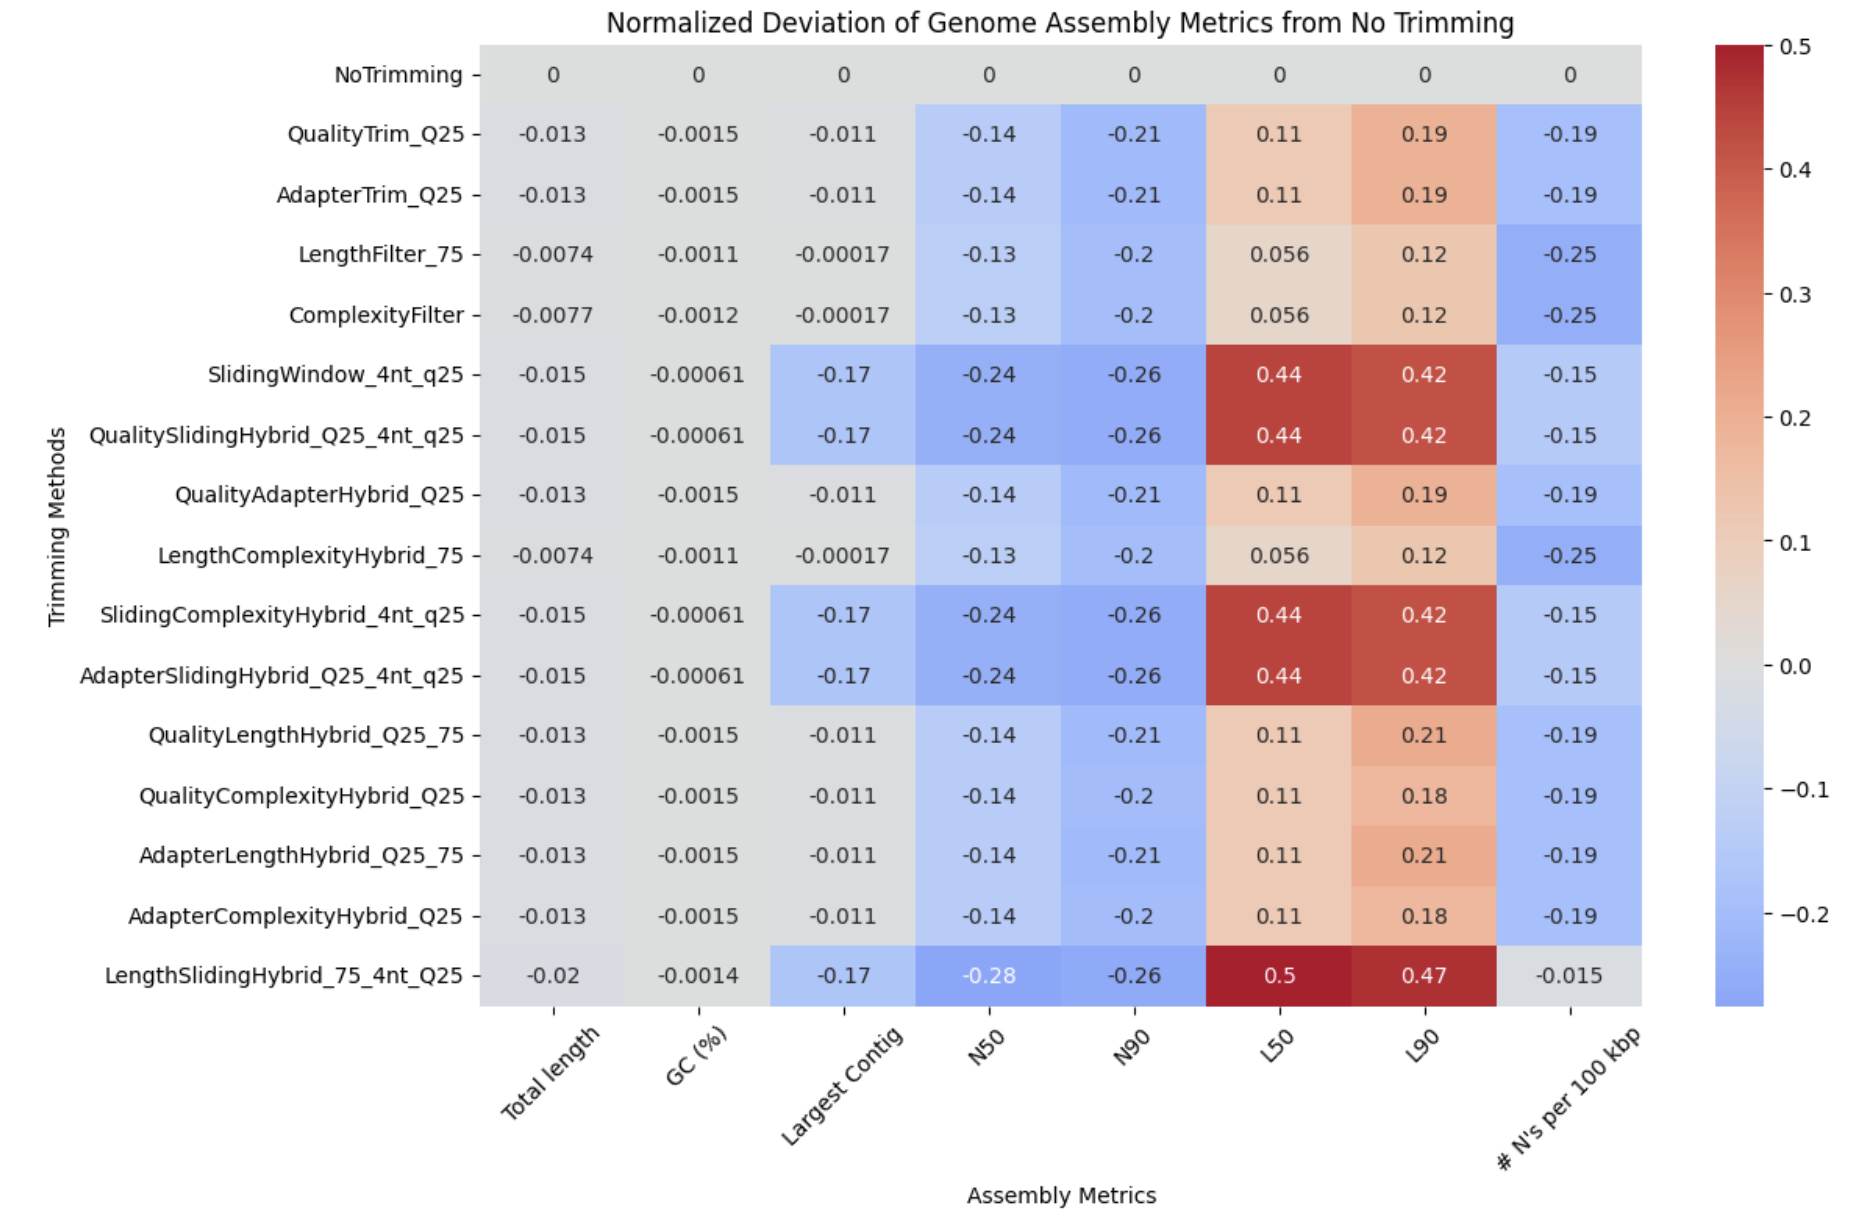
\includegraphics[width=\linewidth]{resources/images/genome_assembly_metrics_heatmap_1.png}
\caption{\textbf{Normalized Deviation of \gls{genome} \gls{metrics} from "No Trimming" — The First \gls{trimming} Strategy}. This \gls{heatmap} illustrates the impact of different \gls{trimming} Methods on various \gls{genome} \gls{metrics}. Darker red indicates a greater positive deviation from \textbf{"No Trimming"}, while darker blue indicates a greater negative deviation. \gls{metrics} include \gls{total length}, \gls{gc}, \gls{largest contigs}, \gls{n50}, \gls{n90}, \gls{l50}, \gls{l90}, and \gls{n's per 100 kbp}.}
\label{fig:genome_assembly_metrics_heatmap_1}
\end{figure}

\textit{The subsequent step involved normalizing the data: this process is described in the \autoref{sec:data_normalization}, where the use of the \autoref{lst:data_norm} is explained in detail.}


A new DataFrame "norm\_deviations" was then generated from a rows\_list consisting of dictionaries, with each dictionary representing a row populated with normalized values.

\textit{The \autoref{fig:genome_assembly_metrics_heatmap_1} was created as a result of execution  the \autoref{lst:heatmap} described in the \autoref{sec:visualization_heatmap}.}



Using the seaborn.heatmap() function, an attempt was made to create a \gls{heatmap} (\autoref{fig:genome_assembly_metrics_heatmap_1}) that eloquently depicts the \gls{deviation} of \gls{genome} \gls{metrics} with respect to the \textbf{"No Trimming"} method. In the spatial configuration of the \gls{heatmap}, rows symbolized the different \gls{trimming} Parameters and columns symbolized the different \gls{genome} \gls{metrics}.

The color of the \gls{heatmap} cells was carefully calibrated to represent the magnitude of \gls{deviation} variances, with the midpoint anchored to zero. Thus, the gradation from red to blue hues indicated the transition from positive to negative \gls{deviation}, respectively. This color scheme was chosen to facilitate intuitive perception of data outliers by providing a sharp visual contrast that highlights the comparative effectiveness of different \gls{trimming} Methods.





\subsection{Evaluating the Trimming Method's Initial Impact} 


\begin{enumerate}
  \item \gls{total length} and \gls{gc} content are largely unaffected (\autoref{fig:genome_assembly_metrics_heatmap_1}) by \gls{trimming} Methods, indicating data consistency and high \gls{sequencing} Quality.
  \item \textbf{Sliding Window \gls{trimming}}, in all its combinations, leads to a significant decrease in \gls{n50} and \gls{n90}, suggesting an over-aggressive approach that negatively impacts \gls{assembly}.
  \item An increase in \gls{l50} and \gls{l90} across several methods indicates more fragmentation and reduced \gls{assembly} Continuity.
  \item \textbf{LengthFilter\_75} and \textbf{ComplexityFilter} methods are noted for their ability to reduce indefinite nucleotides, improving \gls{assembly} Auality and Continuity.
  \item A compromise exists between error reduction and \gls{assembly} Continuity, which needs to be balanced for optimal \gls{assembly} Outcomes.
  \item Further analysis is suggested to assess the compromise between Uncertainty and Continuity \gls{metrics}, possibly through additional hierarchical plotting of the \gls{trimming} Methods.
\end{enumerate}

\subsection{Visual Assessment of Trimming Efficiency} 

\begin{figure}[H]
\centering
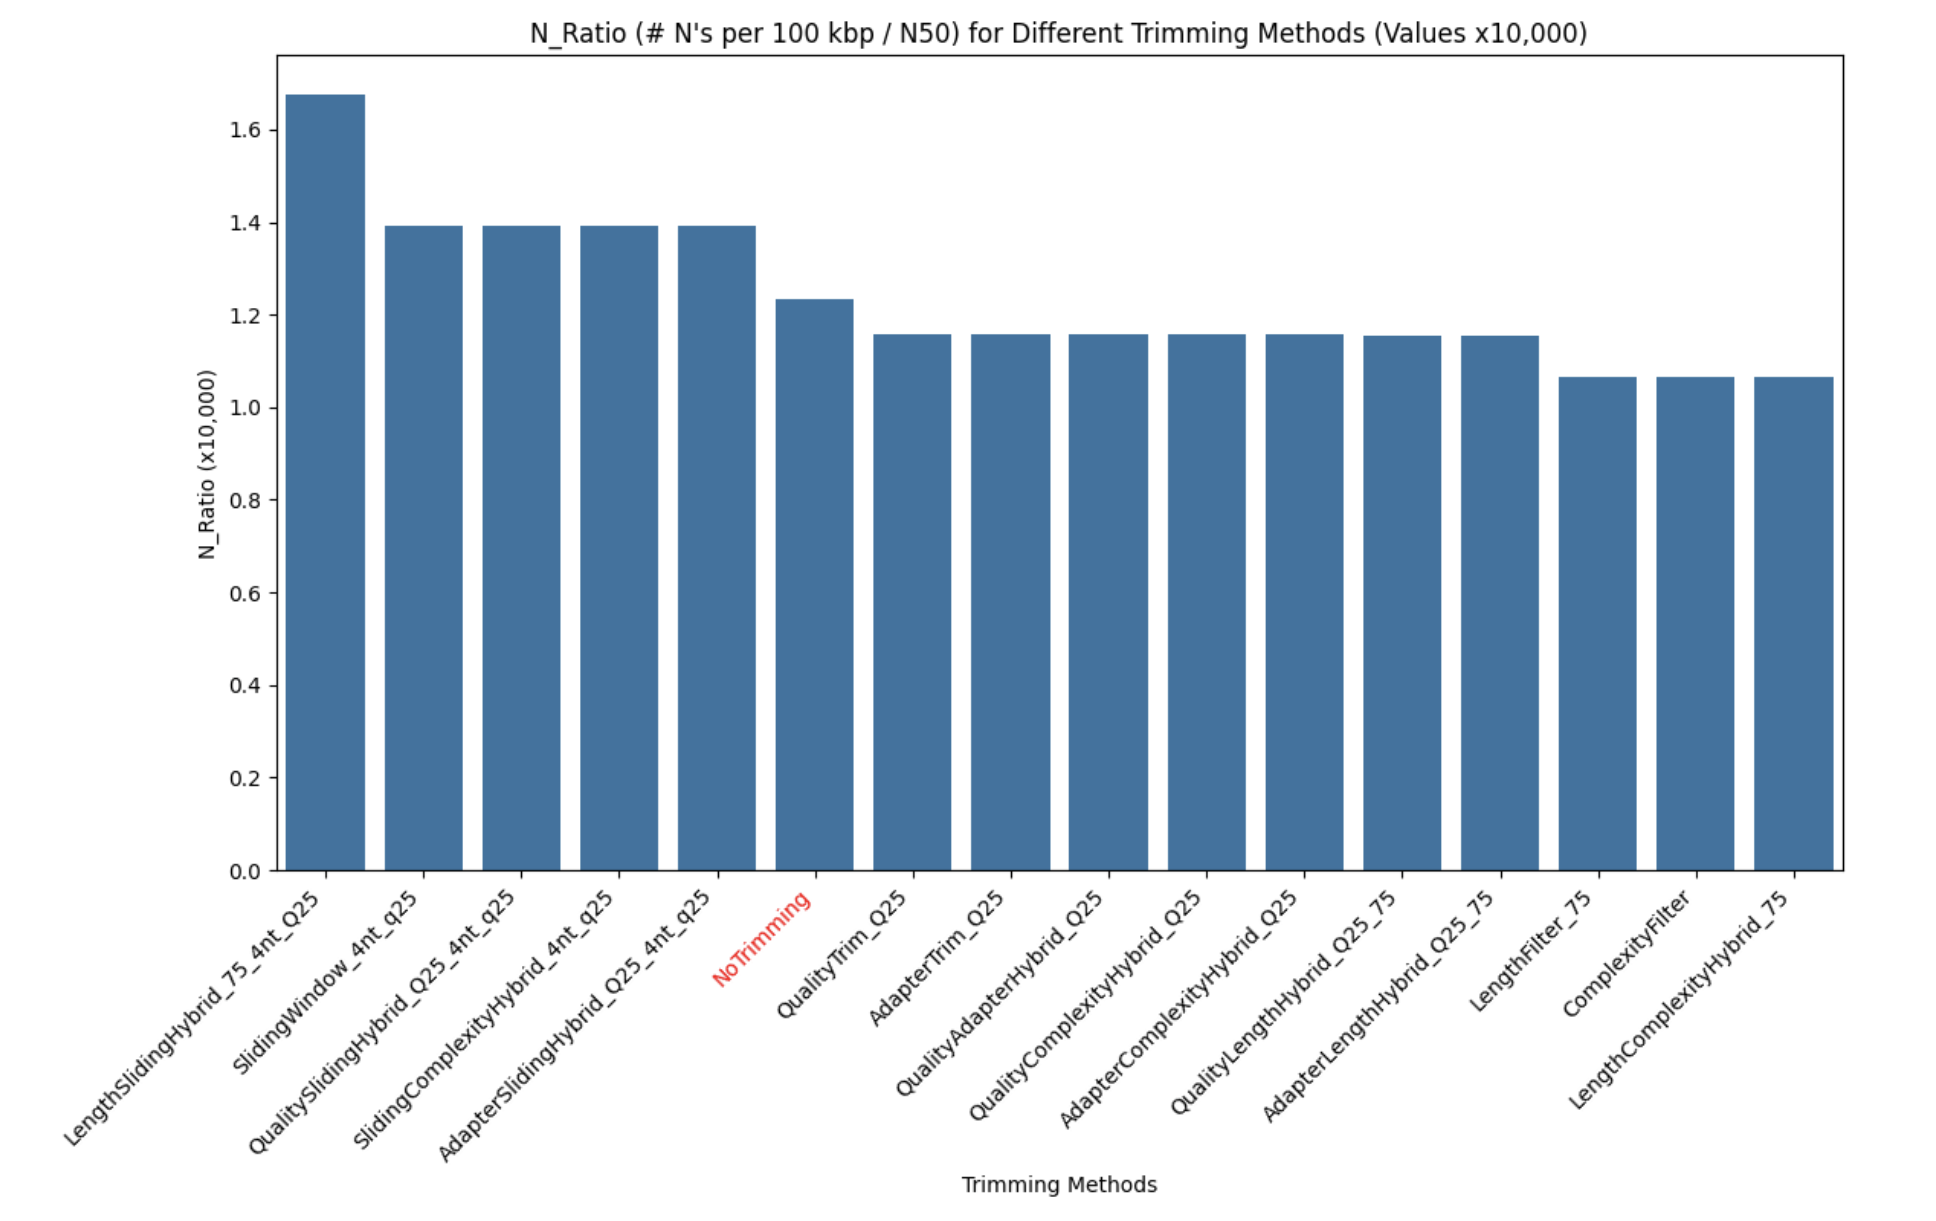
\includegraphics[width=\linewidth]{resources/images/n_ratio_1.png}
\caption{\textbf{The First \gls{trimming} Strategy: the \gls{bar} represents the N ratio — the \gls{n's per 100 kbp} to the \gls{n50} metric for different \gls{trimming} Methods}, with values multiplied by 10,000. The \textbf{'No Trimming'} method serves as a reference point. Each bar represents a different \gls{trimming} Method, and the height of the bar indicates the normalized impact of that method on the \gls{assembly} Quality. A higher bar denotes a method that results in a higher \gls{n's per 100 kbp} relative to the \gls{n50}, suggesting a decrease in \gls{assembly} Quality.}
\label{fig:n_ratio_trim_methods_1}
\end{figure}

\textit{The \autoref{fig:n_ratio_trim_methods_1} was obtained by creating the  N\_ratio, its description is in the  \autoref{sec:calculation_n_ratio}, where the \autoref{lst:n_ratio_calc} performs its computation, and the \autoref{sec:visualization_n_ratio} describes the visualisation of the N\_ratio using the \autoref{lst:n_ratio_visual}.}

\subsection{Refining Trimming Parameters Based on Initial Insights} 

\begin{enumerate}
  \item \gls{trimming} Methods generally outperform (\autoref{fig:n_ratio_trim_methods_1}) \textbf{"No Trimming"} by reducing the \gls{n's per 100 kbp} without compromising \gls{assembly} Continuity, except for methods involving the \textbf{Sliding Window}.
  \item \textbf{LengthFilter\_75}, \textbf{ComplexityFilter}, and their \textbf{hybrid} show the most favorable outcomes in balancing continuity with the reduction of uncertain nucleotides.
\end{enumerate}

To further analyze the impact of \gls{trimming} Methods on \gls{assembly} quality, the following steps are proposed:
\begin{enumerate}
  \item Re-run the software pipeline with a variety of parameters for the \textbf{Sliding Window} and \textbf{Length Filter} methods using The Second \gls{trimming} Strategy (\autoref{sec:2nd_trimming_strategy}).
  \item Parameters for the new run should include:
    \begin{itemize}
      \item 16 different settings for \textbf{Sliding Window} (\autoref{tab:comprehensive_trimming_strategies}).
      \item 6 different settings for \textbf{Length Filter} (\autoref{tab:comprehensive_trimming_strategies}).
    \end{itemize}
  \item Compare the outcomes of these runs with the \textbf{"No Trimming"} to determine the optimal parameters for each method.
\end{enumerate}






\section{The Second Trimming Strategy } \label{sec:2nd_trimming_strategy}


\begin{table}[ht!]
\centering
\caption{The Second Trimming Strategy and Its Impact on Assembly Metrics}
\label{tab:trimming_results_second}
\resizebox{\textwidth}{!}{%
\begin{tabular}{|c|l|r|r|r|r|r|r|r|r|}
\hline
\textbf{\#} & \textbf{Trimming Parameters} & \textbf{Total length} & \textbf{GC (\%)} & \textbf{Largest Contig} & \textbf{N50} & \textbf{N90} & \textbf{L50} & \textbf{L90} & \textbf{\# N's per 100 kbp} \\ \hline
0 & NoTrimming & 4404338 & 65.49 & 209132 & 74608 & 21687 & 18 & 57 & 9.20 \\
1 & SlidingWindow\_4nt\_q15 & 4371714 & 65.47 & 209097 & 66370 & 19392 & 19 & 61 & 7.14 \\
2 & SlidingWindow\_4nt\_q20 & 4355072 & 65.47 & 196013 & 66370 & 16891 & 19 & 66 & 6.92 \\
3 & SlidingWindow\_4nt\_q25 & 4338271 & 65.45 & 173819 & 56417 & 16144 & 26 & 81 & 7.86 \\
4 & SlidingWindow\_4nt\_q30 & 4324613 & 65.42 & 156069 & 45172 & 12240 & 31 & 100 & 4.64 \\
5 & SlidingWindow\_7nt\_q15 & 4386621 & 65.47 & 209097 & 70975 & 20667 & 18 & 59 & 11.52 \\
6 & SlidingWindow\_7nt\_q20 & 4371385 & 65.48 & 196013 & 65416 & 16973 & 20 & 65 & 11.75 \\
7 & SlidingWindow\_7nt\_q25 & 4352562 & 65.46 & 196013 & 64262 & 16735 & 22 & 70 & 7.39 \\
8 & SlidingWindow\_7nt\_q30 & 4335609 & 65.44 & 161559 & 53760 & 15315 & 27 & 84 & 10.41 \\
9 & SlidingWindow\_10nt\_q15 & 4389356 & 65.48 & 209097 & 74525 & 20679 & 18 & 57 & 11.51 \\
10 & SlidingWindow\_10nt\_q20 & 4426558 & 65.49 & 141613 & 49888 & 14028 & 29 & 91 & 20.93 \\
11 & SlidingWindow\_10nt\_q25 & 4359481 & 65.47 & 196013 & 65247 & 16891 & 20 & 66 & 7.15 \\
12 & SlidingWindow\_10nt\_q30 & 4337191 & 65.45 & 141533 & 53760 & 16002 & 27 & 83 & 8.33 \\
13 & SlidingWindow\_20nt\_q15 & 4390654 & 65.47 & 209097 & 70975 & 20679 & 18 & 58 & 9.21 \\
14 & SlidingWindow\_20nt\_q20 & 4377137 & 65.47 & 196013 & 66370 & 19418 & 19 & 61 & 6.91 \\
15 & SlidingWindow\_20nt\_q25 & 4369502 & 65.47 & 196013 & 65416 & 17217 & 21 & 66 & 11.75 \\
16 & SlidingWindow\_20nt\_q30 & 4347271 & 65.46 & 161570 & 64262 & 16677 & 23 & 74 & 10.16 \\
17 & LengthFilter\_50 & 4370507 & 65.41 & 209097 & 65136 & 17421 & 19 & 64 & 6.94 \\
18 & LengthFilter\_75 & 4371727 & 65.42 & 209097 & 65136 & 17421 & 19 & 64 & 6.94 \\
19 & LengthFilter\_100 & 4371227 & 65.42 & 209075 & 64713 & 17421 & 20 & 65 & 6.94 \\
20 & LengthFilter\_150 & 4371488 & 65.42 & 205948 & 64262 & 17416 & 20 & 66 & 6.94 \\
21 & LengthFilter\_200 & 4368193 & 65.42 & 205900 & 64262 & 17416 & 20 & 66 & 7.18 \\
22 & LengthFilter\_250 & 4431464 & 65.42 & 146203 & 41434 & 14197 & 34 & 102 & 16.41 \\
\hline
\end{tabular}%
}
\end{table}


\textit{The data in the \autoref{tab:trimming_results_second} results from reports generated by the second run of the pipeline (\autoref{sec:generated_data}), its extraction with the \autoref{lst:extracting_metrics} calling the \autoref{lst:extraction-function}, and sorting by using the \autoref{lst:sorting_extracted_metrics}, described in the  \autoref{sec:data_extraction}.}

\subsection{Normalization of Comparative Data}

\textit{The subsequent step involved normalizing the data: this process is described in the \autoref{sec:data_normalization}, where the use of the \autoref{lst:data_norm} is explained in detail.}

\subsection{Heatmap Visualization of Refined Data}

\textit{The \autoref{fig:genome_assembly_metrics_heatmap_2} was created as a result of execution the \autoref{lst:heatmap} described in the  \autoref{sec:visualization_heatmap}.}

\begin{figure}[H]
\centering
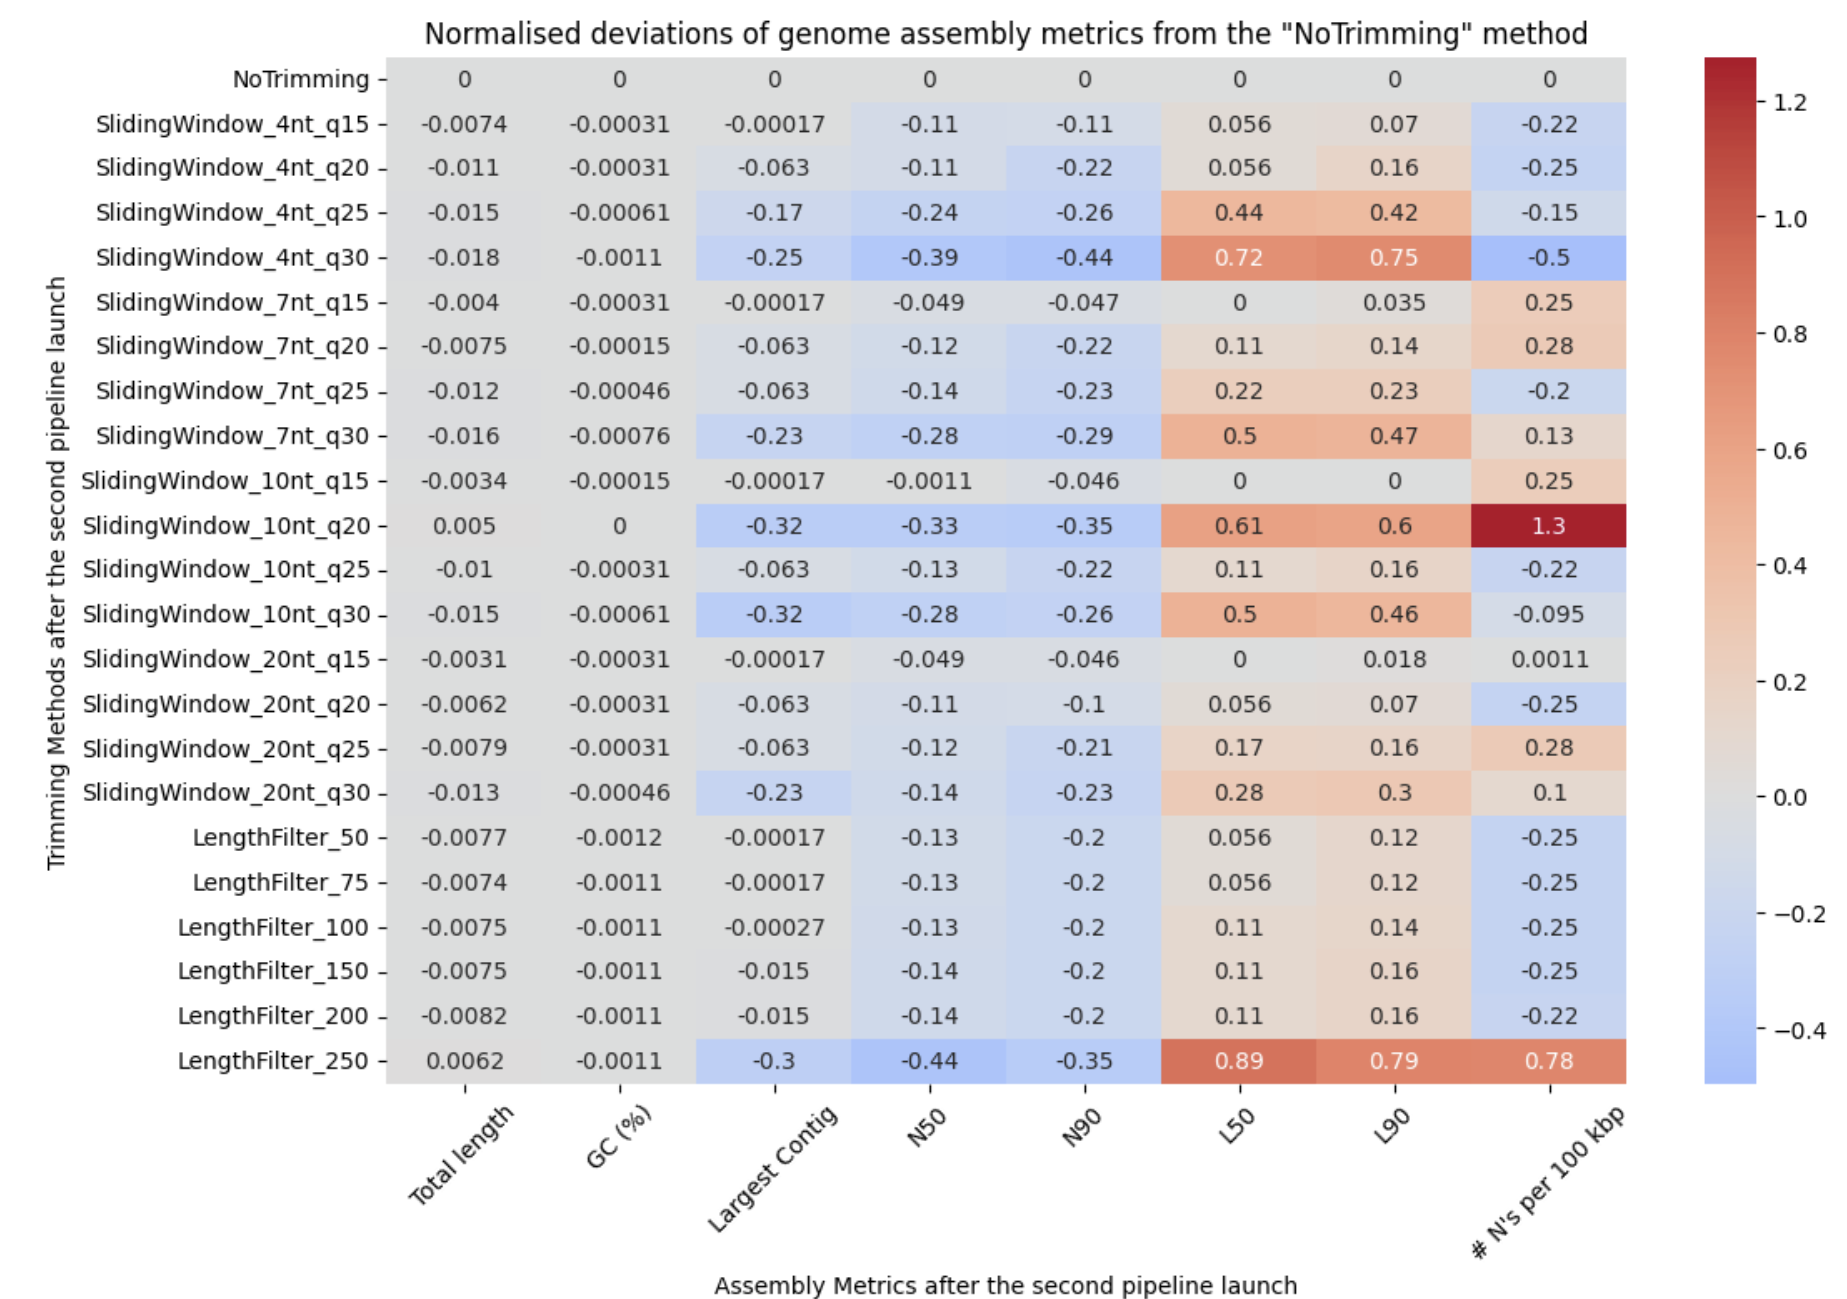
\includegraphics[width=\linewidth]{resources/images/genome_assembly_metrics_heatmap_2.png}
\caption{\textbf{\gls{deviation} of \gls{genome} \gls{metrics} from "No Trimming" — The Second \gls{trimming} Strategy}. This visual representation highlights the impact of different \textbf{Sliding Window} and \textbf{Length Filter} parameters on \gls{metrics} such as \gls{total length}, \gls{gc}, \gls{largest contigs}, \gls{n50}, \gls{n90}, \gls{l50}, \gls{l90}, and \gls{n's per 100 kbp}. Notably, certain parameters show a marked decrease in \gls{n50} and increase in \gls{l50}, \gls{l90}, suggesting a compromise between \gls{trimming} Stringency and \gls{assembly} Continuity.}
\label{fig:genome_assembly_metrics_heatmap_2}
\end{figure}



\subsection{Assessment of Refined Trimming Parameters}

\begin{enumerate}
  \item As the \gls{n's per 100 kbp} decreases (\autoref{fig:genome_assembly_metrics_heatmap_2}), there is a corresponding decrease in \gls{n50} and \gls{n90}, and an increase in \gls{l50} and \gls{l90}, highlighting a consistent pattern across \gls{trimming} Methods.
  \item Some \gls{trimming} Methods, such as \textbf{SlidingWindow\_7nt\_q15}, lead to an increased number of N's without significantly altering other parameters, indicating a poor \gls{trimming} Performance.
  \item Extreme cases, like \textbf{SlidingWindow\_10nt\_q20} and \textbf{LengthFilter\_250}, cause a drastic reduction in \gls{assembly} Quality.
\end{enumerate}

To further understand the impact of \gls{trimming} Methods:
\begin{enumerate}
  \item An additional plot (\autoref{fig:n_ratio_after_second_pipeline}) will be created to rank the \gls{trimming} Methods by the ratio of the frequency of N's to the \gls{n50} metric, thereby establishing a hierarchy of method effectiveness.
\end{enumerate}

\subsection{Bar Chart Analysis of N Ratio Improvements} 

\textit{The \autoref{fig:n_ratio_after_second_pipeline} was obtained by creating the N\_ratio, its description is in the  \autoref{sec:calculation_n_ratio}, where the \autoref{lst:n_ratio_calc} performs its computation, and the \autoref{sec:visualization_n_ratio} describes the visualisation of the N\_ratio using the  \autoref{lst:n_ratio_visual}.}

\begin{figure}[h!]
\centering
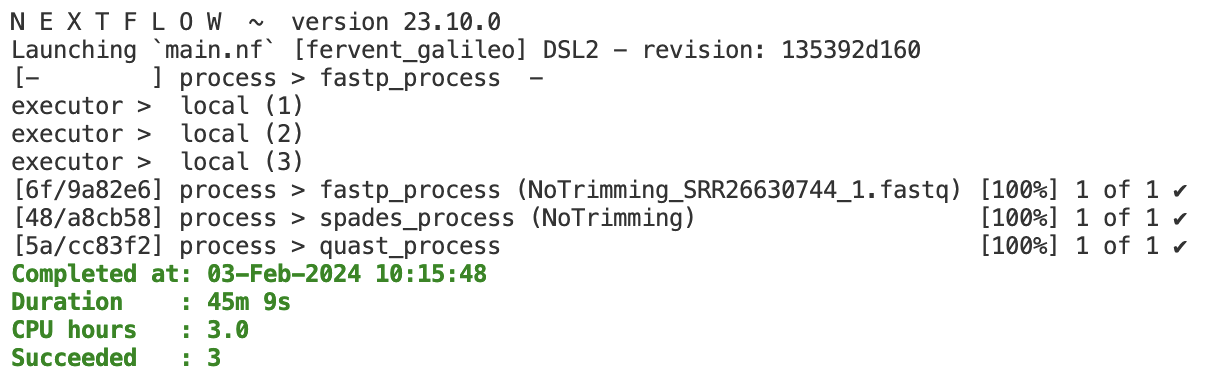
\includegraphics[width=\linewidth]{resources/images/nextflow_output.png}
\caption{\textbf{An example of an output of the Nextflow pipeline execution}, version 23.10.0, showcasing the completion of various bioinformatics processes. The workflow includes processes such as 'fastp\_process', 'spades\_process', and 'quast\_process' with inputs like 'NoTrimming\_SRR26630744\_1.fastq'. The execution was completed on 03-Feb-2024 at 10:15:48, taking a total duration of 45 minutes and 9 seconds, consuming 3.0 CPU hours, and successfully completing three processes for the single "NoTrimming" Method.}
\label{fig:nextflow_output}
\end{figure}

\begin{figure}[H]
\centering
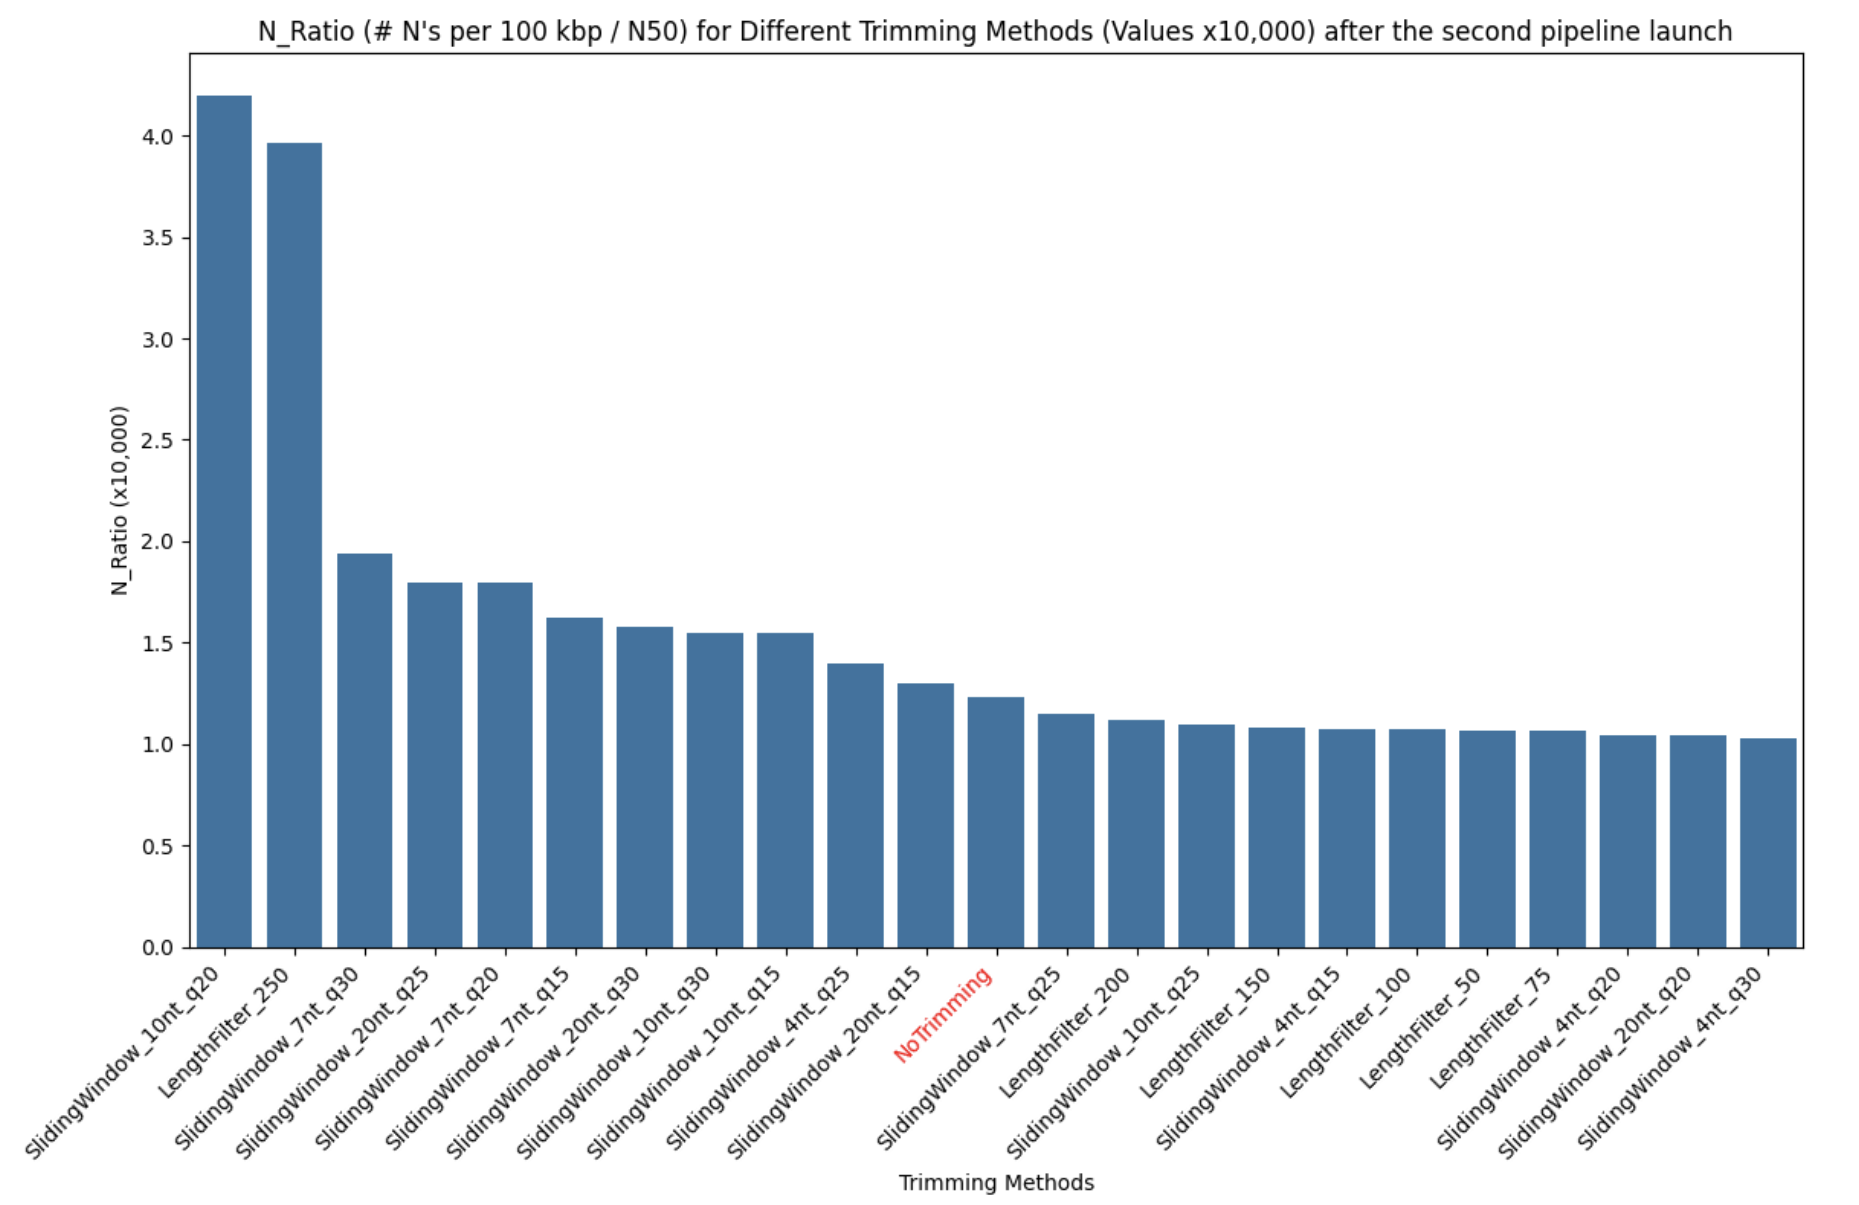
\includegraphics[width=\linewidth]{resources/images/n_ratio_2.png}
\caption{\textbf{The Second \gls{trimming} Strategy: the \gls{bar} showing the N\_Ratio, which is the \gls{n's per 100 kbp} divided by the \gls{n50} metric, for different \gls{trimming} Methods} following the second pipeline run. The values are multiplied by 10,000 to facilitate comparison. The \textbf{'No Trimming'} method serves as a benchmark. A higher bar denotes a method that results in a higher \gls{n's per 100 kbp} relative to the \gls{n50}, suggesting a decrease in \gls{assembly} Quality.}
\label{fig:n_ratio_after_second_pipeline}
\end{figure}



\subsection{Critical Analysis of Parameter Refinement}

\begin{enumerate}
  \item Certain parameters (\autoref{fig:n_ratio_after_second_pipeline}) of the \textbf{Sliding Window} method, previously considered suboptimal, have shown improved \gls{assembly} Quality upon re-evaluation, even outperforming the previously favored \textbf{LengthFilter\_75} in some instances.
  \item Conversely, some parameters of the initially superior \textbf{Length Filter} method, such as \textbf{LengthFilter\_250}, may not be advantageous, indicating the significance of parameter selection within each method.
\end{enumerate}

Further Insights and Steps:

\begin{enumerate}
  \item The importance of the \gls{trimming} Method's parameters has been experimentally validated, influencing the quality of \gls{assembly}.
  \item The iterative use of the pipeline has refined our understanding of which \gls{trimming} Methods and parameters yield the best \gls{assembly} Quality.
  \item A new visualization approach is proposed using \gls{scatter} (\autoref{fig:length_filter_variation}, \autoref{fig:3d_scatter_sliding_window}) to analyze the variance in \gls{assembly} Quality across different parameters within the \textbf{Sliding Window} and \textbf{Length Filter} methods.
  \item Specifically for \textbf{Length Filter}, the 2D \gls{scatter} (\autoref{fig:length_filter_variation}) will be created to illustrate the relationship between its parameters and the metrics \gls{n50} and the \gls{n's per 100 kbp}.
\end{enumerate}



\subsection{Visualizing Optimal Trimming Outcomes}



\begin{figure}[H]
\centering
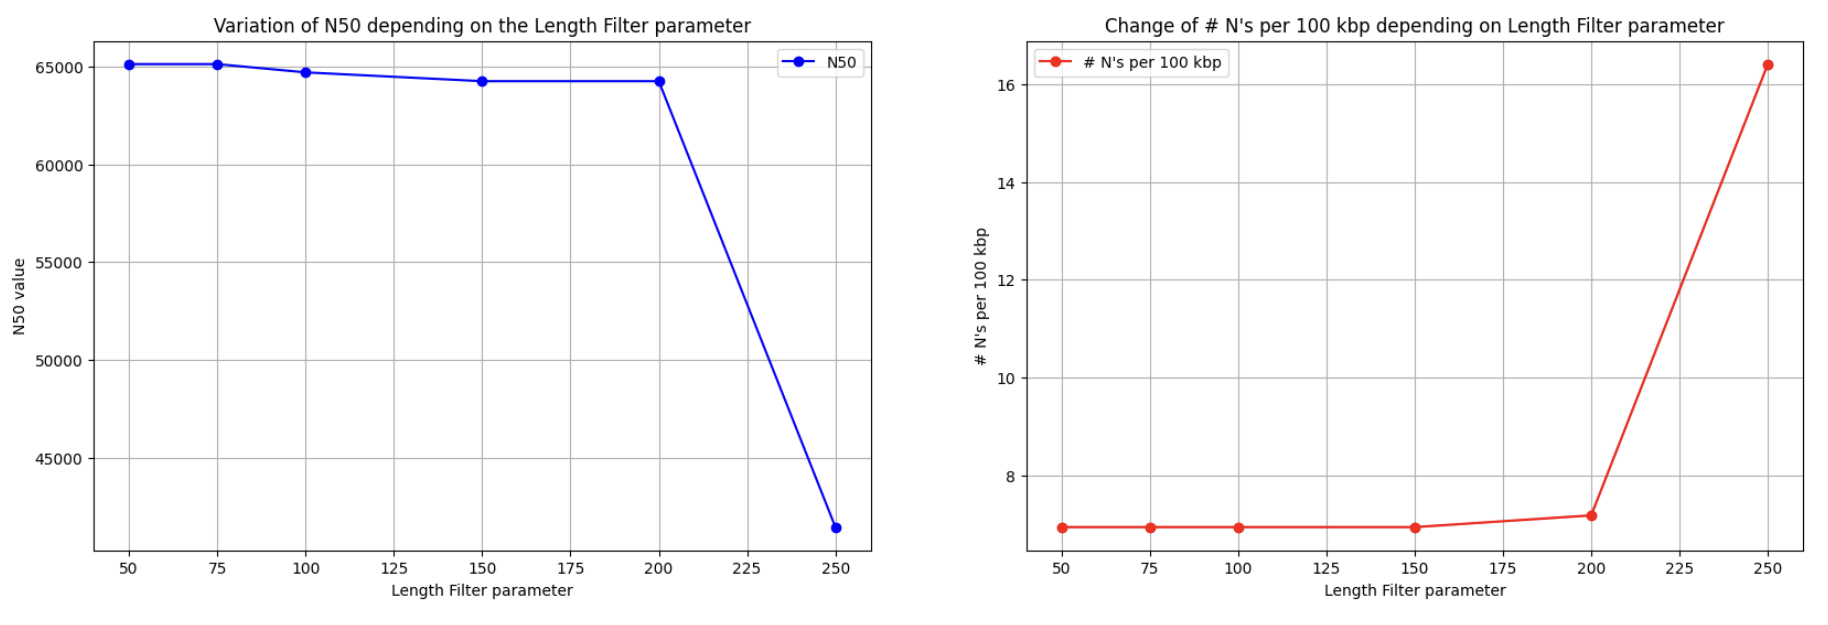
\includegraphics[width=\linewidth]{resources/images/length_filter_variation.png}
\caption{\textbf{The dual \gls{scatter} illustrate the variation of the \gls{n50} metric (left) and the change in the \gls{n's per 100 kbp} (right) as a function of the Length Filter parameter}. The \gls{n50} value remains relatively stable across a range of parameters but sharply decreases after a certain threshold. Conversely, the \gls{n's per 100 kbp} stays consistent before dramatically increasing, indicating a critical parameter value beyond which the \textbf{Length Filter} negatively impacts the \gls{assembly}.}
\label{fig:length_filter_variation}
\end{figure}

\textit{The \autoref{fig:length_filter_variation} was created by using the \autoref{lst:scatter_plot} described in the  \autoref{sec:length_filter_trimming} and in the  \autoref{sec:length_filter_trimming_visualisation}. And the \autoref{fig:3d_scatter_sliding_window} was created by using the \autoref{lst:3d_scatter_plot} described in the  \autoref{sec:sliding_window_trimming} and in the \autoref{sec:sliding_window_trimming_visualisation}. The \autoref{fig:3d_scatter_sliding_window} depicts just a screenshot of the visual program MetricsExtractor, which interactively allows researches to find the best of the best metrics (\autoref{sec:sliding_window_trimming_visualisation}).}


\begin{SCfigure}
  \centering
  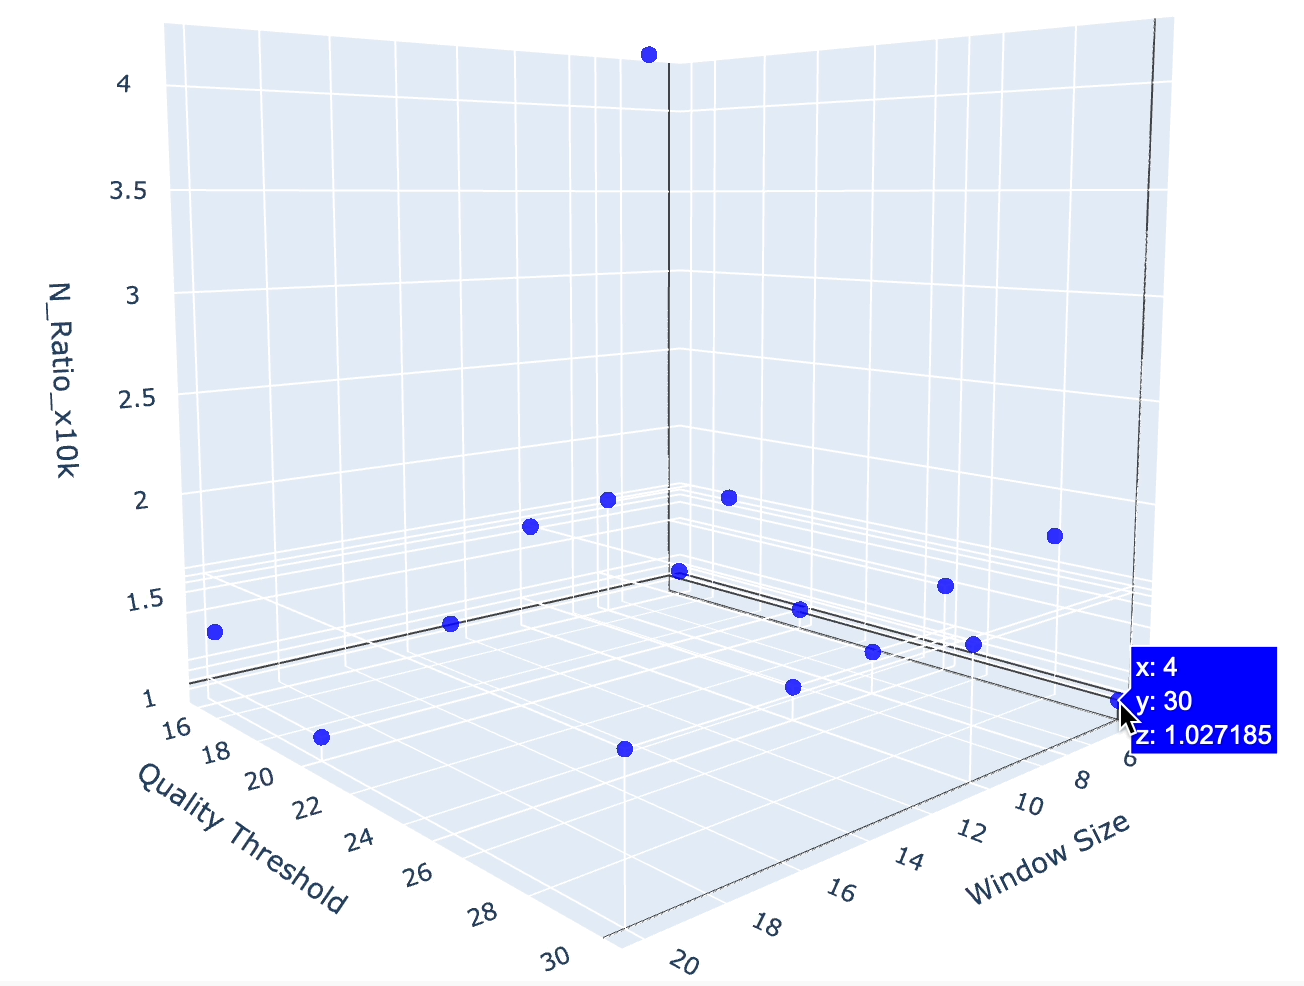
\includegraphics[width=0.48\textwidth]{resources/images/3d_scatter_sliding_window.png}
  \caption{\textbf{The 3D \gls{scatter} representing the N\_Ratio\_x10k of the Sliding Window \gls{trimming} Method as a function of its parameters}, specifically window size and quality threshold. The plot points are distributed across the three-dimensional space defined by these two parameters and the resulting N\_Ratio\_x10k, highlighting the complex relationship between \gls{trimming} Method parameters and the impact on \gls{assembly} Quality.}
  \label{fig:3d_scatter_sliding_window}
\end{SCfigure}



\subsection{Final Evaluation of Trimming Strategy Efficacy}

\begin{enumerate}
  \item The \gls{scatter}s (\autoref{fig:length_filter_variation}, \autoref{fig:3d_scatter_sliding_window}) reveal an inverse relationship between the \gls{n50} metric and the \gls{n's per 100 kbp}, illustrating the impact of the \textbf{Length Filter} parameter on \gls{assembly} Quality.
  \item Parameters in the range of 50 to 75 for the Length Filter method are indicated to potentially enhance \gls{assembly} Quality.
  \item A proposal is made to re-run the pipeline with \textbf{Length Filter} parameters around 50-75 to possibly improve \gls{assembly} Quality further.
  \item For the \textbf{Sliding Window} method, the 3D \gls{scatter} (\autoref{fig:3d_scatter_sliding_window}) is suggested to analyze the N\_Ratio\_x10k against its varying parameters, necessitating data filtering to select for \textbf{Sliding Window} parameters exclusively.
  \item The interactive 3D \gls{scatter} allows us to examine each data point alongside its corresponding X (window size), Y (mean quality), and Z (N\_Ratio\_x10k) values, illustrating the \gls{trimming} Method's parameter effects on \gls{assembly} Quality.
  \item The point with the lowest Z value on the plot indicates the optimal parameters for the \textbf{Sliding Window} method that achieve the best balance between the \gls{n's per 100 kbp} and \gls{n50}, suggesting a superior \gls{assembly} Quality.
  \item Initiating a third pipeline run with parameters near this optimal point may potentially refine the quality of \gls{genome} \gls{trimming} even further.
\end{enumerate}





\section{The Third Trimming Strategy }  \label{sec:3rd_trimming_stratrgy}


\begin{table}[ht!]
\centering
\caption{The Third Trimming Strategy and Its Impact on Assembly Metrics}
\label{tab:trimming_results_third}
\resizebox{\textwidth}{!}{%
\begin{tabular}{|c|l|r|r|r|r|r|r|r|r|}
\hline
\textbf{\#} & \textbf{Trimming Parameters} & \textbf{Total length} & \textbf{GC (\%)} & \textbf{Largest Contig} & \textbf{N50} & \textbf{N90} & \textbf{L50} & \textbf{L90} & \textbf{\# N's per 100 kbp} \\ \hline
0 & SlidingWindow\_3nt\_q30 & 4302594 & 65.40 & 139540 & 38864 & 10691 & 34 & 111 & 1.86 \\
1 & SlidingWindow\_4nt\_q30 & 4310805 & 65.42 & 156069 & 45172 & 12240 & 31 & 100 & 4.64 \\
2 & SlidingWindow\_4nt\_q29 & 4314963 & 65.43 & 161279 & 49758 & 12487 & 29 & 94 & 6.49 \\
3 & SlidingWindow\_5nt\_q30 & 4315324 & 65.43 & 161302 & 45552 & 12261 & 31 & 98 & 6.49 \\
4 & LengthFilter\_30 & 4321024 & 65.41 & 209097 & 65136 & 17421 & 19 & 64 & 6.94 \\
5 & LengthFilter\_35 & 4321024 & 65.41 & 209097 & 65136 & 17421 & 19 & 64 & 6.94 \\
6 & LengthFilter\_40 & 4321012 & 65.41 & 209097 & 65136 & 17421 & 19 & 64 & 6.94 \\
7 & LengthFilter\_45 & 4321017 & 65.41 & 209097 & 65136 & 17421 & 19 & 64 & 6.94 \\
8 & LengthFilter\_50 & 4321006 & 65.41 & 209097 & 65136 & 17421 & 19 & 64 & 6.94 \\
9 & LengthFilter\_55 & 4321006 & 65.41 & 209097 & 65136 & 17421 & 19 & 64 & 6.94 \\
\hline
\end{tabular}%
}
\end{table}

\textit{The data in the \autoref{tab:trimming_results_third} results from reports generated by the third run of the pipeline (\autoref{sec:generated_data}), its extraction with the \autoref{lst:extracting_metrics} calling the \autoref{lst:extraction-function}, and sorting by using the \autoref{lst:sorting_extracted_metrics}, described in the  \autoref{sec:data_extraction}.}

\textit{The \autoref{fig:length_filter_variation_2} was created by using the \autoref{lst:scatter_plot} described in the  \autoref{sec:length_filter_trimming} and in the  \autoref{sec:length_filter_trimming_visualisation}. And the \autoref{fig:n_ratio_3} was obtained by creating the N\_ratio, its description is in the  \autoref{sec:calculation_n_ratio}, where the \autoref{lst:n_ratio_calc} performs its computation, and the \autoref{sec:visualization_n_ratio} describes the visualisation of the N\_ratio using the  \autoref{lst:n_ratio_visual}.}



\subsection{Comparative Overview of Genome Assembly Metrics}

\begin{figure}[H]
    \centering
    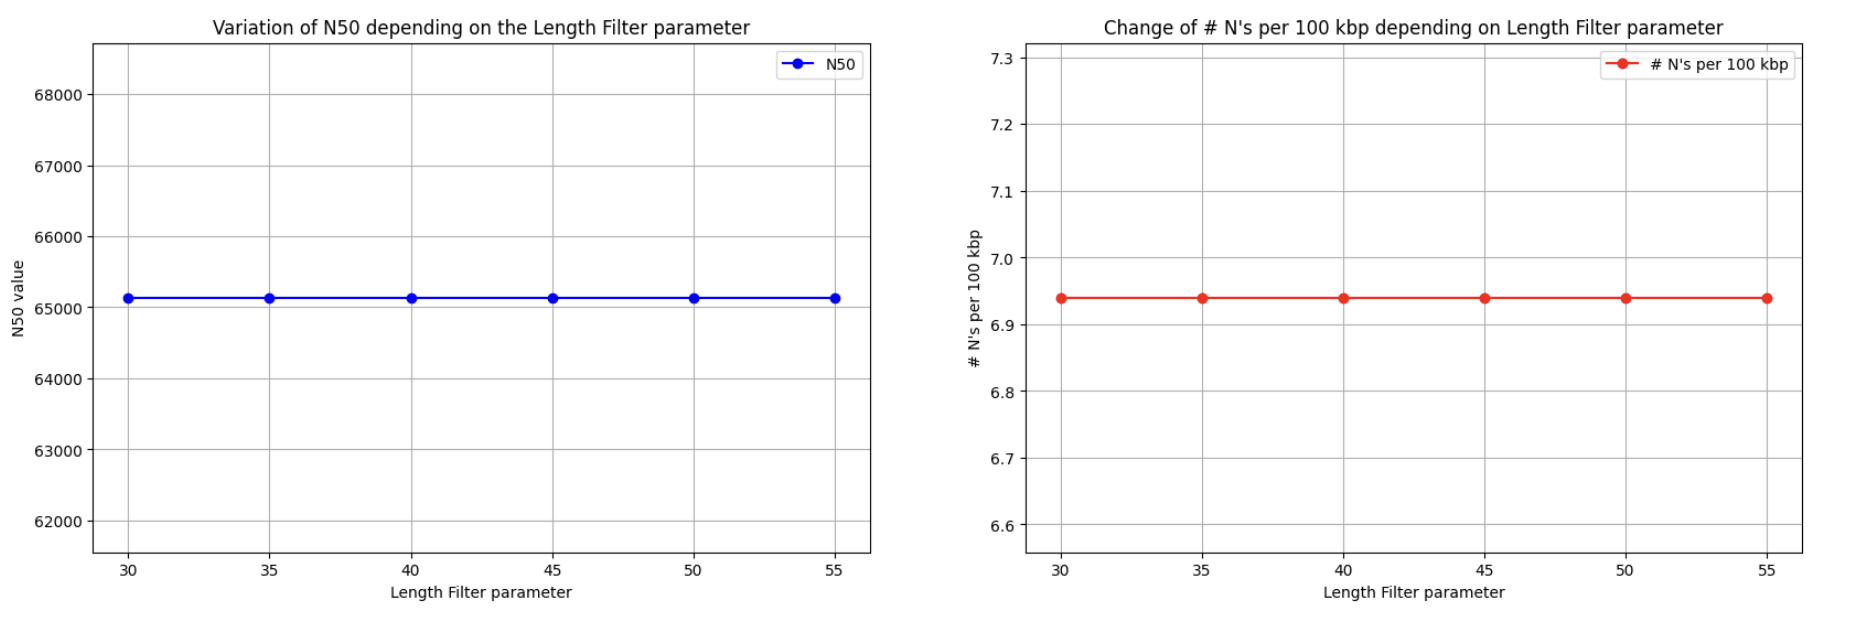
\includegraphics[width=0.7\linewidth]{resources/images/length_filter_variation_2.png}
    \caption{\textbf{Two \gls{scatter}s depicting the variation of the \gls{n50} metric and the change in the \gls{n's per 100 kbp} as functions of the Length Filter parameter.} The left plot shows \gls{n50} values remaining stable across different parameters, while the right plot illustrates a consistent \gls{n's per 100 kbp}, independent of the \textbf{Length Filter} parameter changes. These trends suggest that within the examined parameter range, the \textbf{Length Filter} has a negligible effect on both the continuity and the gap size of the \gls{assembly}.}
    \label{fig:length_filter_variation_2}
    
    \vspace{1cm}
    
    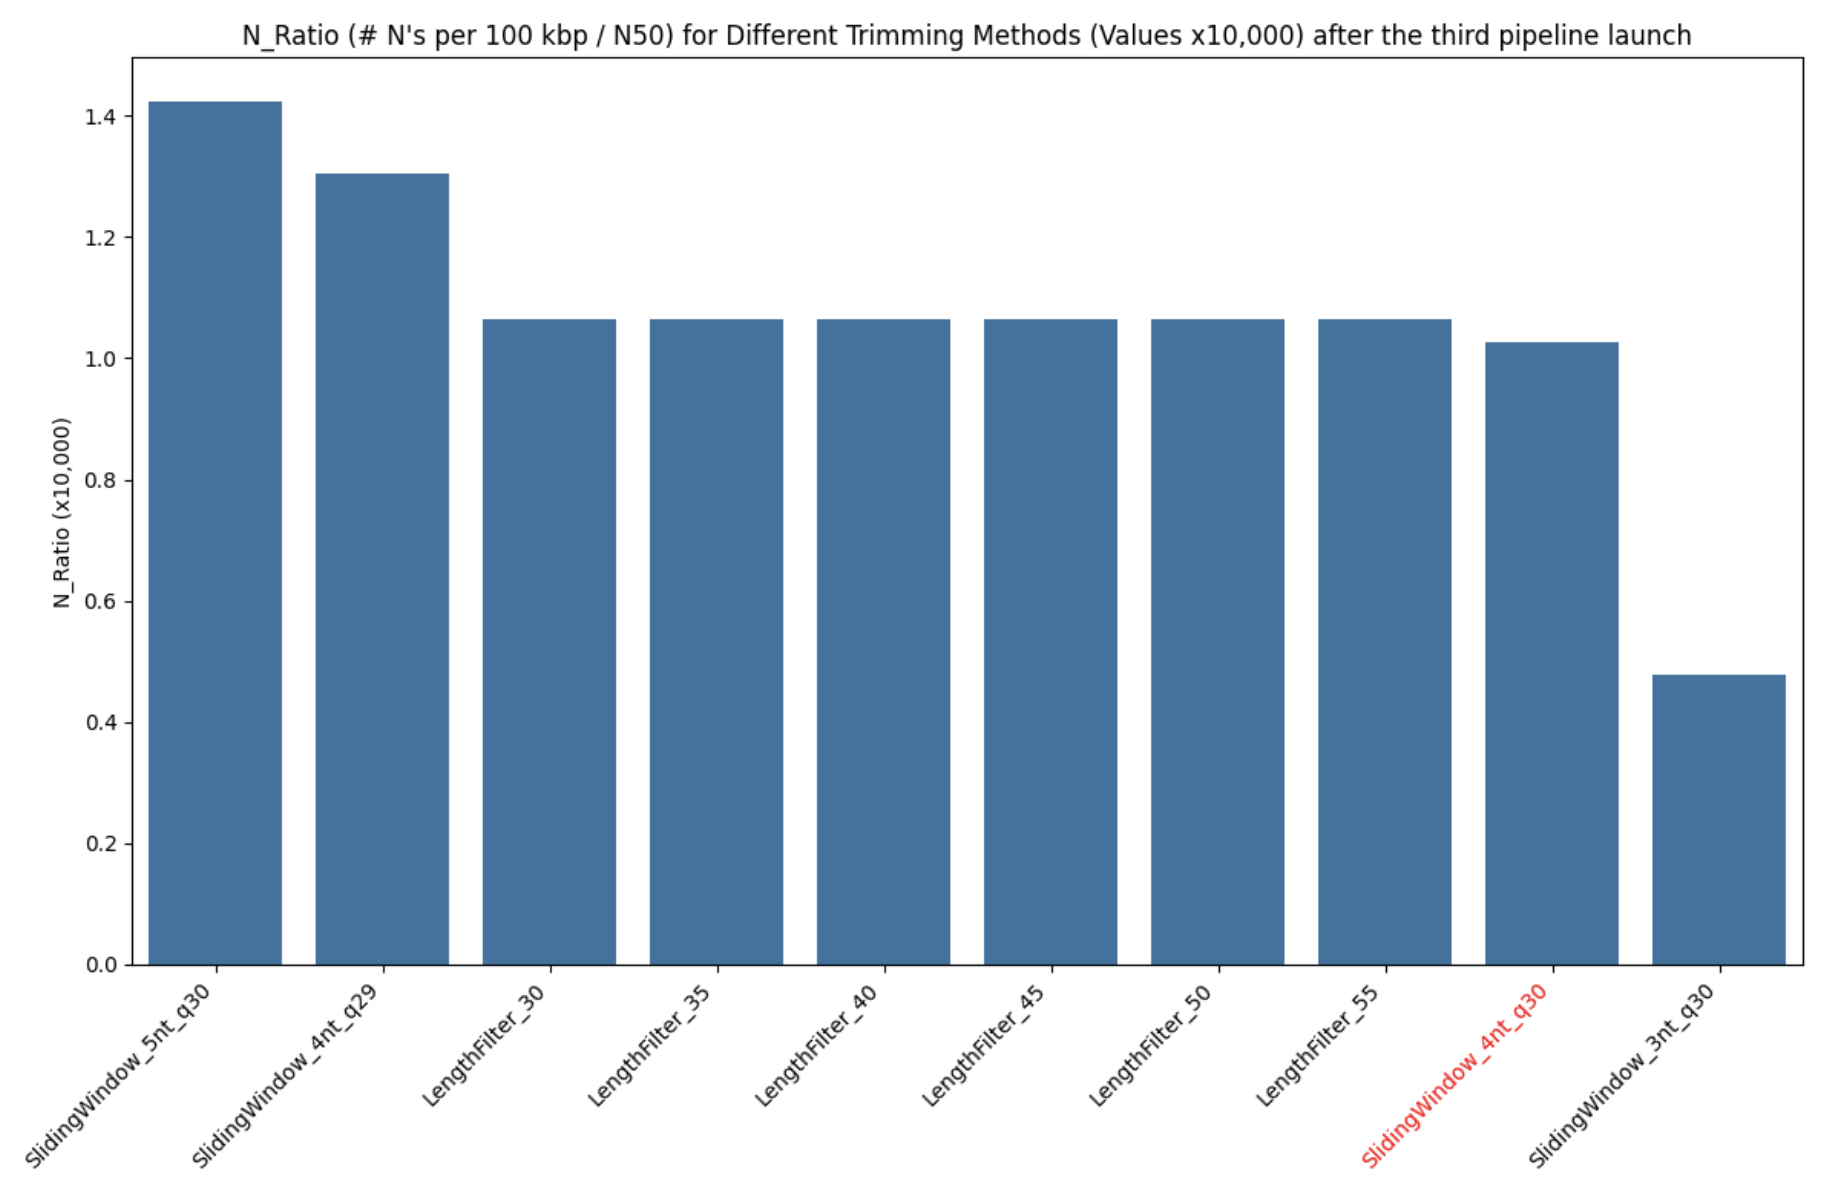
\includegraphics[width=0.7\linewidth]{resources/images/n_ratio_3.png}
    \caption{\textbf{\gls{bar}s showing the N\_Ratio (\gls{n's per 100 kbp} / \gls{n50}) for different \gls{trimming} Methods after the third pipeline run}, multiplied by 10,000. The bars represent various methods, including \textbf{Sliding Window} and \textbf{Length Filter}, with their respective parameter values. The significant decrease in the N\_Ratio for certain parameters indicates a more favorable outcome in \gls{assembly} Quality.}
    \label{fig:n_ratio_3}
\end{figure}



\subsection{Conclusive Insights on Trimming Efficacy}

\begin{enumerate}
    \item The analysis of the graph (\autoref{fig:length_filter_variation_2}) indicates that modifying the \gls{trimming} Method parameters to values near their previously identified optimum does not yield improvement. Consequently, the initial hypothesis was not corroborated by the results.
    \item \autoref{fig:n_ratio_3}: our hypothesis was confirmed, leading to the discovery of an improved data \gls{trimming} method using the \textbf{SlidingWindow\_3nt\_q30} parameters.
\end{enumerate}


\section{A Comparative Analysis}

\begin{figure}[!ht]
    \centering
    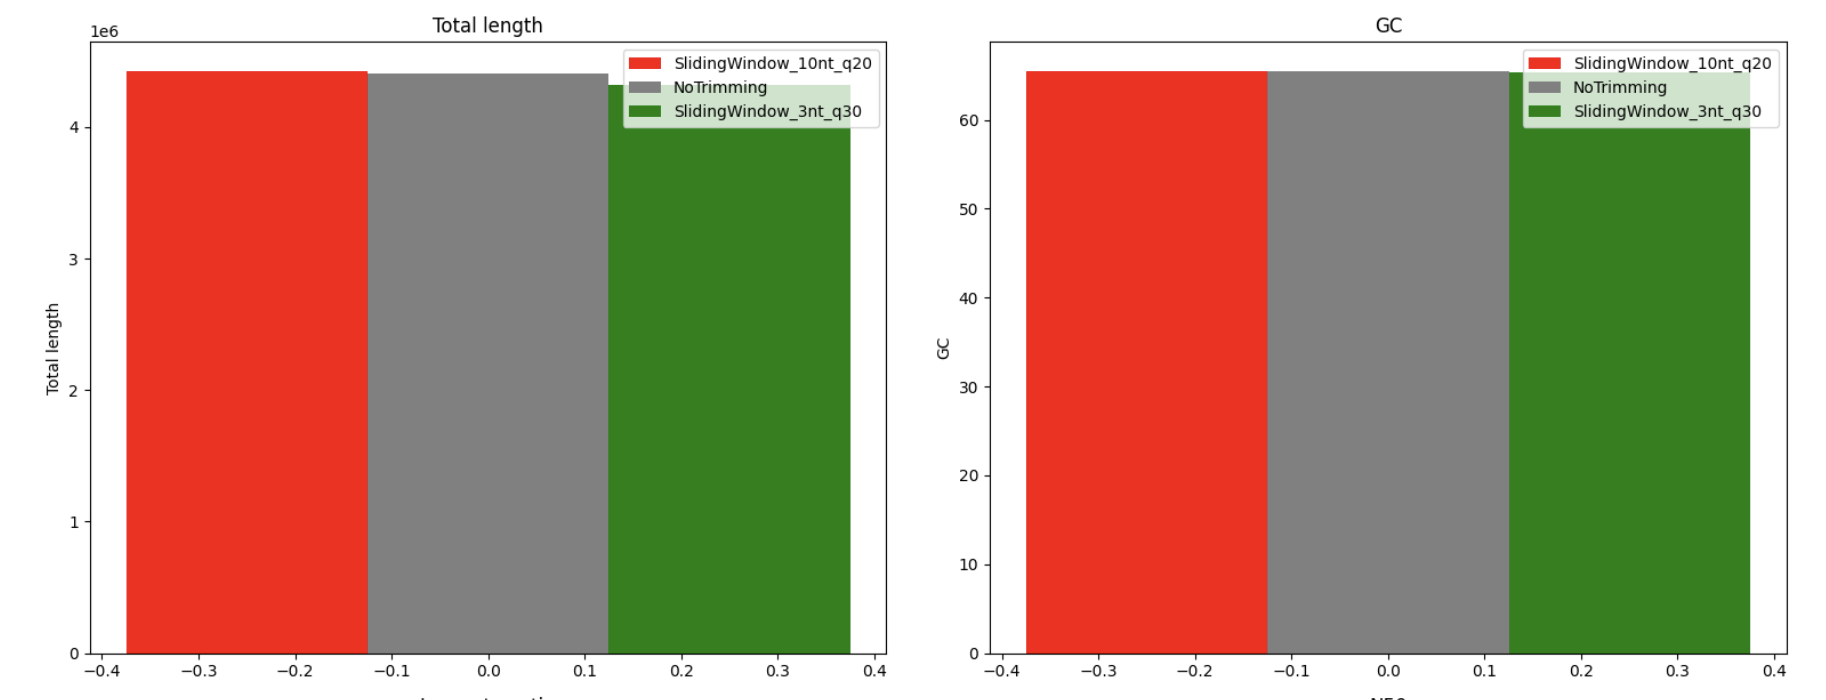
\includegraphics[width=0.8\textwidth]{resources/images/total_length_gc.png}
    \caption{\textbf{\gls{total length} and \gls{gc}} - worst/best}
    \label{fig:total_length_gc}
\end{figure}

\begin{figure}[!ht]
    \centering
    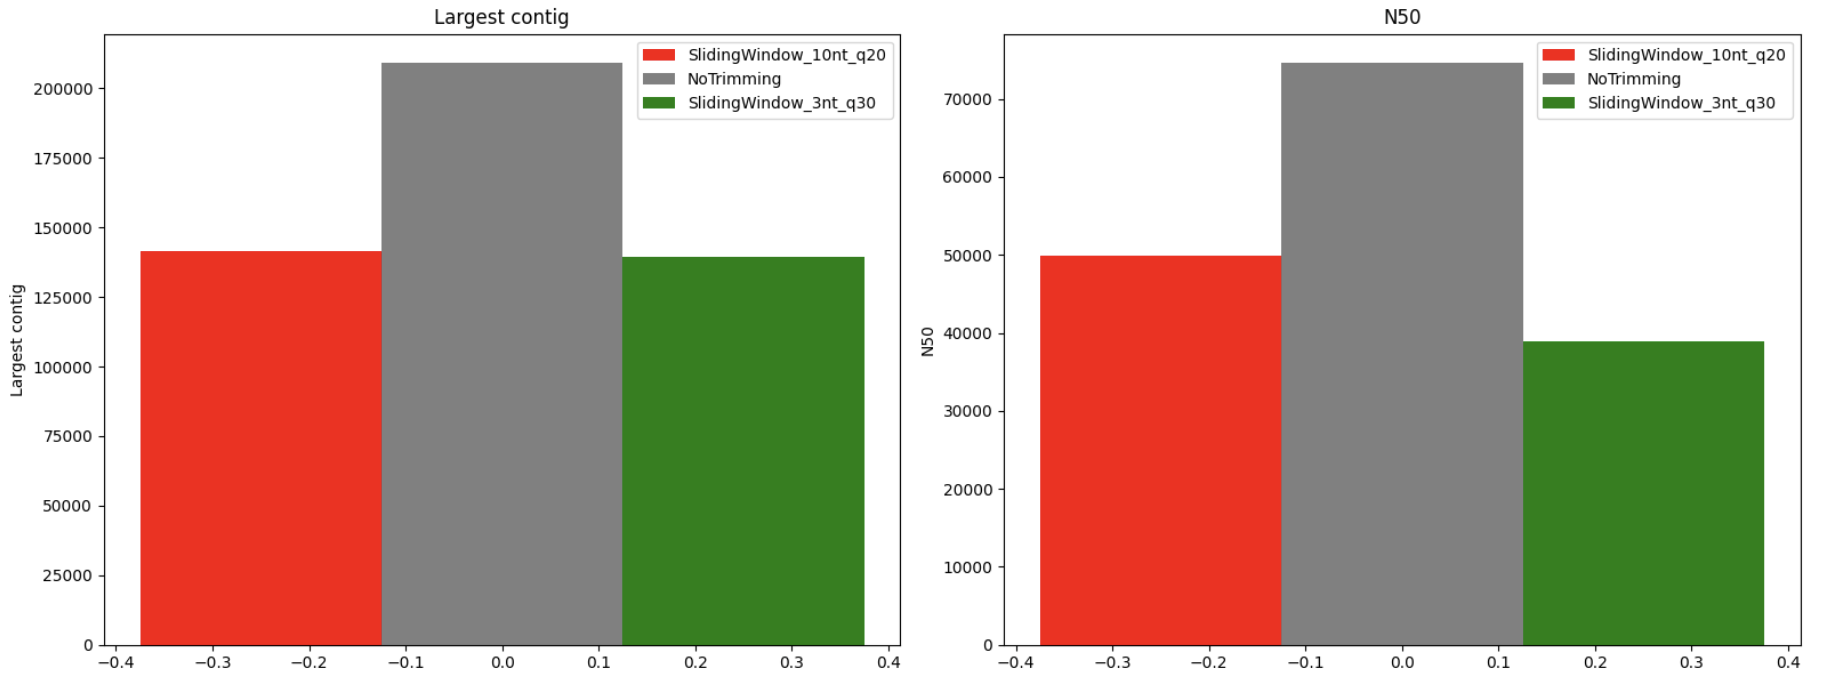
\includegraphics[width=0.8\textwidth]{resources/images/largest_contig_n50.png}
    \caption{\textbf{\gls{largest contigs} and \gls{n50}} - worst/best}
    \label{fig:largest_contig_n50}
\end{figure}

\begin{figure}[!ht]
    \centering
    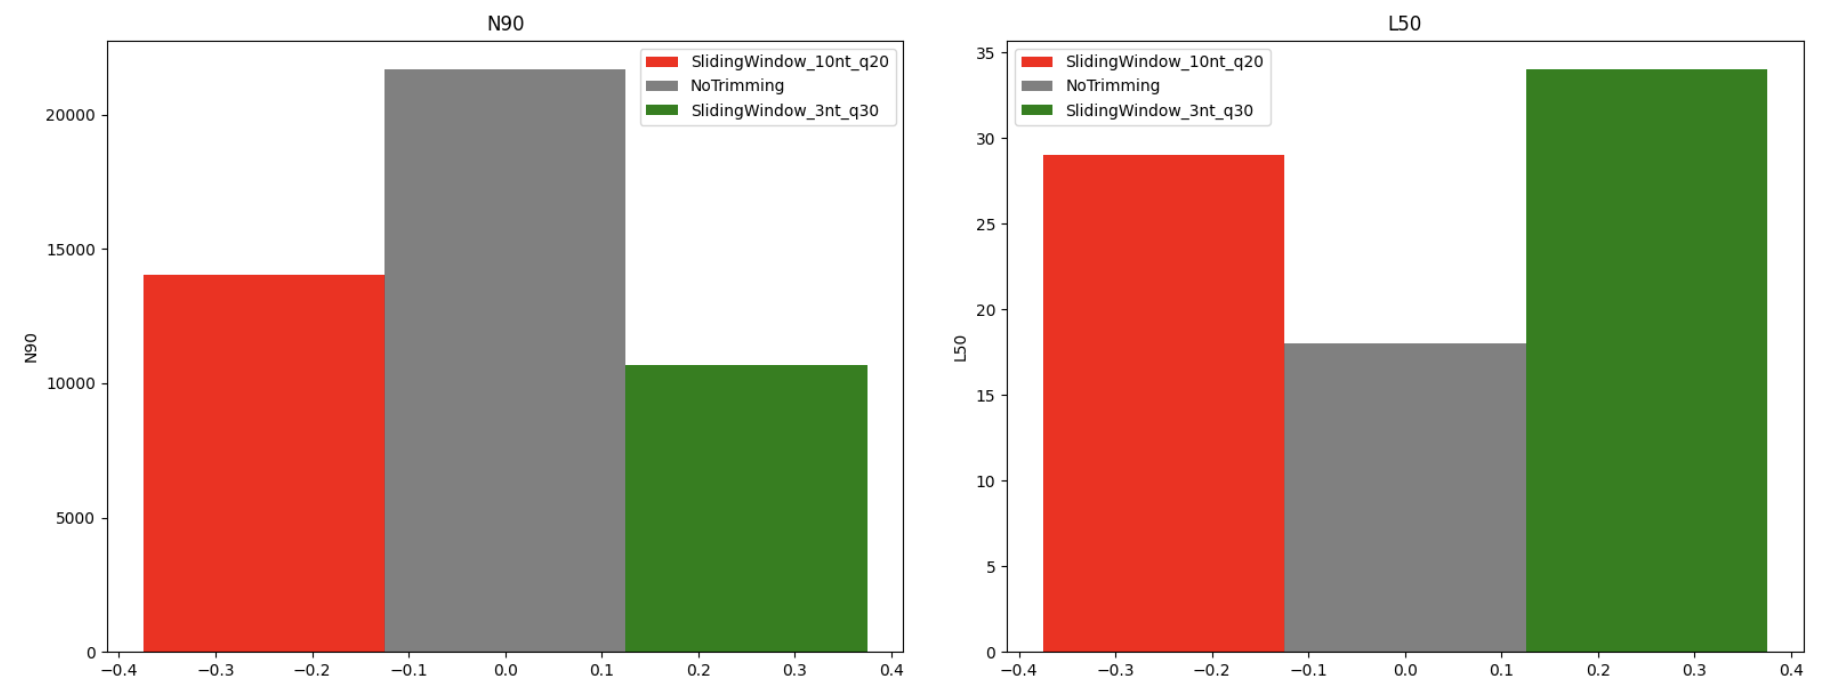
\includegraphics[width=0.8\textwidth]{resources/images/n90_l50.png}
    \caption{\textbf{\gls{n90} and \gls{l50}} - worst/best}
    \label{fig:n90_l50}
\end{figure}

\begin{figure}[!ht]
    \centering
    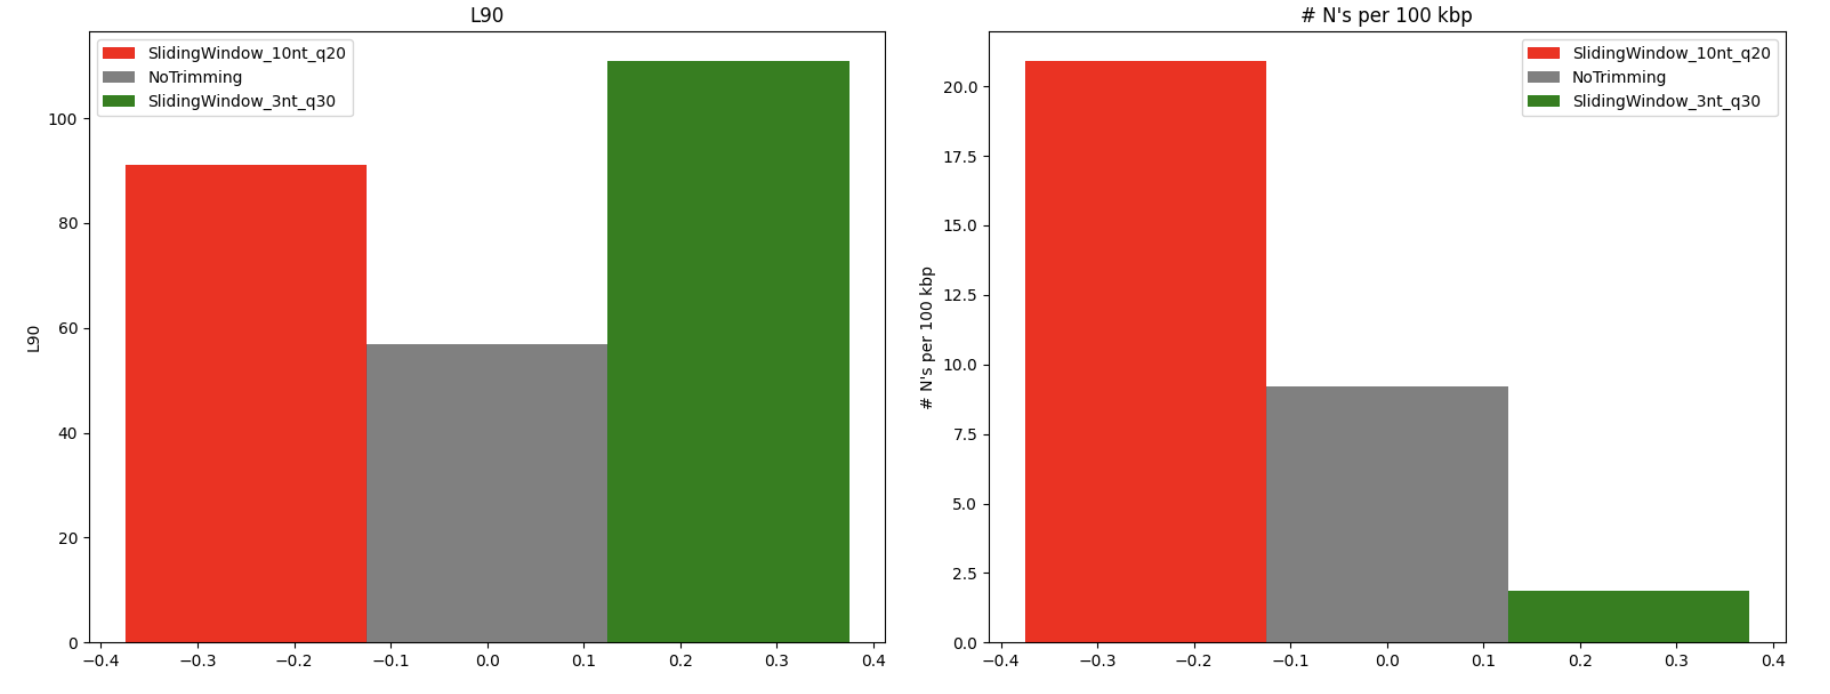
\includegraphics[width=0.8\textwidth]{resources/images/l90_ns_per_100kbp.png}
    \caption{\textbf{\gls{l90} and \gls{n's per 100 kbp}} - worst/best}
    \label{fig:l90_ns_per_100kbp}
\end{figure}


\begin{enumerate}
    \item{Comparative \gls{bar}s of \gls{assembly} Metrics for different \gls{trimming} Methods. Demonstrative comparison of the effects of three \gls{trimming} Methods on different metrics assessing the quality of \gls{assembly}. The best \gls{trimming} Method found (\textbf{SlidingWindow\_3nt\_q30}) demonstrates the advantage of using the pipeline.}
    \item Through iterative execution of the pipeline and intermediate data processing, we identified the most and least effective data \gls{trimming} Methods (\autoref{fig:l90_ns_per_100kbp}), depicted in green and red respectively, against the \textbf{"No Trimming"} (gray) scenario.
    \item The optimal \gls{trimming}  Method, \textbf{SlidingWindow\_3nt\_q30}, demonstrated the lowest N\_Ratio value among all tested, indicating the highest efficiency in reducing the \gls{n's per 100 kbp}  relative to \gls{n50}.
    \item The improvement factor for the best \gls{trimming} Method over the no-trimming scenario was \textbf{4.95} in terms of \gls{n's per 100 kbp} , showcasing significant enhancement in data quality. The \gls{n50}  indicator decreased by \textbf{1.9} times compared to when \gls{trimming}  was not used.
\end{enumerate}